
\documentclass[12pt, a4paper, oneside]{report}

% ── Encodage & langue ──────────────────────────────────────
\usepackage[utf8]{inputenc}
\usepackage[T1]{fontenc}
\usepackage[french]{babel}

% ── Mise en page ───────────────────────────────────────────
\usepackage[
  top=2.5cm, bottom=2.5cm,
  left=3cm,  right=2.5cm
]{geometry}
\usepackage{setspace}
\onehalfspacing

% ── Polices & typographie ──────────────────────────────────
\usepackage{lmodern}
\usepackage{microtype}

% ── Mathématiques ─────────────────────────────────────────
\usepackage{amsmath, amssymb, amsfonts}

% ── Graphiques & figures ──────────────────────────────────
\usepackage{graphicx}
\usepackage{float}
\usepackage{subcaption}
\graphicspath{{figures/}}

% ── Tableaux ──────────────────────────────────────────────
\usepackage{booktabs}
\usepackage{multirow}
\usepackage{array}
\usepackage{longtable}

% ── Liens hypertexte ──────────────────────────────────────
\usepackage[
  colorlinks = false,
  hidelinks
]{hyperref}

% ── Bibliographie ─────────────────────────────────────────
\usepackage[
  backend  = biber,
  style = numeric,
  sorting  = none
]{biblatex}
\addbibresource{references.bib}

% ── En-têtes & pieds de page ──────────────────────────────
\usepackage{fancyhdr}
\pagestyle{fancy}
\fancyhf{}
\fancyhead[L]{\small\leftmark}
\fancyhead[R]{\small\thepage}
\renewcommand{\headrulewidth}{0.4pt}

% ── Style des chapitres ───────────────────────────────────
\usepackage{titlesec}
\titleformat{\chapter}[display]
  {\normalfont\Large\bfseries}
  {\chaptertitlename\ \thechapter}{12pt}{\Huge}
\titlespacing*{\chapter}{0pt}{-20pt}{30pt}

% ── Listes d'acronymes ────────────────────────────────────
\usepackage{acronym}

% ── Code source ───────────────────────────────────────────
\usepackage{listings}
\lstset{
  basicstyle   = \ttfamily\small,
  breaklines   = true,
  frame        = single,
  captionpos   = b,
  numbers      = left,
  numberstyle  = \tiny,
  keywordstyle = \bfseries,
  commentstyle = \itshape,
  stringstyle  = \ttfamily
}

% ── Algorithmes ───────────────────────────────────────────
\usepackage{algorithm}
\usepackage{algpseudocode}

% ── Divers ────────────────────────────────────────────────
\usepackage{lipsum}
\usepackage{pdfpages}
\usepackage{enumitem}

% ============================================================
%   INFORMATIONS DU MÉMOIRE
% ============================================================
\newcommand{\titre}{Vectorization Automatique d'Images Matricielles par Deep Learning}
\newcommand{\domainedetude}{Mathématiques et Informatique}
\newcommand{\specialite}{Ingénierie de Systèmes d'Information \& Logiciels}
\newcommand{\auteurA}{BITAM Amir}
\newcommand{\auteurB}{AITHAMOUDI Zakaria}
\newcommand{\encadreur}{ABDELLAHOUM Hamza}
\newcommand{\juryA}{????}
\newcommand{\juryB}{????}
\newcommand{\annee}{2025/2026}


% ============================================================
\begin{document}

\pagenumbering{gobble}

% ============================================================
%   PAGE DE GARDE
% ============================================================
\begin{titlepage}
  \centering

  
  % \includegraphics[width=3cm]{logo_usthb.png}\\[0.5cm]

  {\small
    République Algérienne Démocratique et Populaire\\
    Ministère de l'Enseignement Supérieur et de la Recherche Scientifique\\[0.3cm]
  }
  

  {\bfseries
    Higher Institute of Sciences\\
    [0.2cm]
  }

   
\includegraphics[width=6cm]{his_logo.png}\hfill

  {\large\bfseries Projet de fin d'étude}\\[0.1cm]
  {\bfseries En:} \domainedetude\\[0.1cm]
  {\bfseries Spécialité :} \specialite\\[0.1cm]
  {\bfseries Intitulé :}\\[0.1cm]

  \rule{\linewidth}{1.5pt}\\[0.4cm]
  {\Huge\bfseries \titre}\\[0.4cm]
  \rule{\linewidth}{1.5pt}\\[1.5cm]

  \begin{minipage}[t]{0.45\textwidth}
    \textbf{Encadré par :}\\
    \encadreur\\[0.5cm]
    \textbf{Membres du Jury :}\\
    \juryA\\
    \juryB
  \end{minipage}
  \hfill
  \begin{minipage}[t]{0.45\textwidth}
    \raggedleft
    \textbf{Présenté par :}\\
    \auteurA\\
    \auteurB\\[0.5cm]
    \textbf{Soutenu le :}\\
    ??/07/2026
  \end{minipage}

  \vfill
  Année universitaire : \annee
\end{titlepage}

% ============================================================
%   PAGES LIMINAIRES
% ============================================================
\pagenumbering{roman}
\setcounter{page}{1}

% ── Remerciements ─────────────────────────────────────────
\chapter*{Remerciements}
\addcontentsline{toc}{chapter}{Remerciements}

Nous tenons à exprimer notre profonde gratitude envers Allah, le Tout-Puissant, pour
nous avoir accordé la force, la patience et la persévérance nécessaires pour mener à bien ce
projet de fin d'étude.

Nous remercions sincèrement notre encadreur \textbf{\encadreur} pour sa précieuse
guidance, son soutien constant et ses précieux conseils tout au long de ce projet.

Nos vifs remerciements s'adressent également aux membres du jury \textbf{\juryA}
et \textbf{\juryB} pour avoir accepté d'évaluer notre travail.

% TODO : compléter les remerciements

% ── Dédicace ─────────────────────────────────────────────
\chapter*{Dédicace}
\addcontentsline{toc}{chapter}{Dédicace}

% TODO : insérer les dédicaces personnelles

\newpage

% ── Résumé ───────────────────────────────────────────────
\chapter*{Résumé}
\addcontentsline{toc}{chapter}{Résumé}

Nous proposons dans le cadre de notre projet de fin d'études un modèle d'IA qui traite
le zoom et le dézoom dans les images numériques. En zoomant sur une image de taille
donnée, sa qualité est souvent altérée et l'image peut devenir pixélisée. Notre travail consiste
à améliorer ces images en augmentant leur qualité.

En ce qui concerne le dézoom, en réduisant les dimensions de l'image, il faut minimiser
le nombre de pixels tout en préservant l'esthétique de l'image.

Nous avons créé un modèle CNN avec une architecture adaptée, piloté par des
métaheuristiques (algorithme génétique) permettant de sélectionner les paramètres optimaux
afin d'obtenir de bonnes performances avec un nombre minimal de paramètres.

\bigskip\noindent
\textbf{Mots-clés :} Redimensionnement d'images, Super Résolution, Réseaux de Neurones
Convolutifs (CNN), Algorithme Génétique, Métaheuristiques, PSNR, SSIM.

\newpage

% ── Abstract ──────────────────────────────────────────────
\chapter*{Abstract}
\addcontentsline{toc}{chapter}{Abstract}

% TODO : traduire le résumé en anglais

\bigskip\noindent
\textbf{Keywords:} Image Resizing, Super Resolution, Convolutional Neural Networks (CNN),
Genetic Algorithm, Metaheuristics, PSNR, SSIM.

\newpage

% ── Acronymes ─────────────────────────────────────────────
\chapter*{Liste des Acronymes}
\addcontentsline{toc}{chapter}{Liste des Acronymes}

\begin{acronym}[SRCNN]
  \acro{XML}{eXtensible Markup Language}
  \acro{SVG}{Scalable Vector Graphics}
  \acro{GA}{Genetic Algorithm}
  \acro{CNN}{Convolutional Neural Networks}
  \acro{PSNR}{Peak Signal to Noise Ratio}
  \acro{HR}{High Resolution}
  \acro{LR}{Low Resolution}
  \acro{SSIM}{Structural SIMilarity}
  \acro{SRCNN}{Super Resolution Convolutional Neural Network}
  \acro{SRGAN}{Super Resolution Generative Adversarial Network}
  \acro{MAE}{Mean Absolute Error}
  \acro{MSE}{Mean Squared Error}
  \acro{ReLU}{Rectified Linear Unit}
  \acro{ResNet}{Residual Network}
  \acro{SE}{Squeeze-and-Excitation}
  \acro{CAR}{Content Adaptive Resampler}
  \acro{FARF}{Feature Augmented Random Forest}
  \acro{DRDN}{Deep Residual Dense Network}
  \acro{EDSAN}{Enhanced Dense Space Attention Network}
  \acro{PPI}{Pixels Per Inch}
\end{acronym}

\newpage

\setcounter{secnumdepth}{5}
\setcounter{tocdepth}{5}
\tableofcontents

\listoffigures

\listoftables

% ============================================================
%   CORPS DU MÉMOIRE
% ============================================================
\pagenumbering{arabic}
\setcounter{page}{1}

% ============================================================
%   INTRODUCTION GÉNÉRALE
% ============================================================
\chapter*{Introduction Générale}
\addcontentsline{toc}{chapter}{Introduction Générale}
\markboth{Introduction Générale}{Introduction Générale}

Le traitement d'images est un domaine de recherche important qui trouve des applications
dans divers domaines tels que la médecine, la surveillance, la sécurité, la robotique,
l'automobile, etc.

% TODO : compléter l'introduction générale

L'un des problèmes les plus courants dans ce domaine est la qualité de l'image qui peut
être altérée lorsqu'elle est agrandie ou réduite en taille.

\bigskip
Ce mémoire est organisé comme suit :
\begin{itemize}
  \item \textbf{Chapitre 1 :} État de l'art — revue de littérature sur le redimensionnement
        d'images et les approches existantes.
  \item \textbf{Chapitre 2 :} Approche proposée — architecture des modèles CNN et
        sélection des hyperparamètres par méta heuristiques.
  \item \textbf{Chapitre 3 :} Expérimentations et Résultats — évaluation quantitative
        et qualitative avec comparaisons.
\end{itemize}

% ============================================================
%   CHAPITRE 1 — ÉTAT DE L'ART
% ============================================================
\chapter{État de l'Art}

\section{Introduction}
L'intelligence artificielle par le biais de l'apprentissage automatique a imposé un changement de paradigme dans de nombreux domaines\cite{dhar2024paradigm}, en particulier l'informatique et ses différentes disciplines. La vision par ordinateur est un parfait exemple de ce changement de paradigme, où la spécialité s'est dirigé de l'application d'algorithmes "naïf" à l'utilisation de réseaux de neurones pour le traitement et l'extraction d'informations de l'image, cette évolution dans les techniques utilisées par la vision par ordinateur est illustré dans l'évolution de la vectorisation d'images.  Dans ce chapitre, nous exposerons d'abord les concepts clés à la vectorisation d'images, à l'apprentissage automatique, et les architectures utilisées tout au long de ce travail, ceci nous permettra de mieux appréhender ensuite les travaux effectués sur le sujet.
\section{Définitions liées à la vectorisation d'images}
Dans cette section nous tenterons de définir les termes et concepts lié à la transformation d'image matricielles en images vectorielles, dite, vectorisation d'images. En soulignant notamment la différence entre les images dites matricielles et vectorielles. En opposant ainsi les deux types d'images nous pourrons mieux cerner la motivation derrière ce travail et pourquoi la vectorisation d'image constitue un exercice complexe de la vision par ordinateur.

  \subsection{Images matricielles}
  Les images matricielles pourrait être décrites de la même manière que  \cite{gonzalez2018digital} le fait, soit des fonction bidimensionnelles $f(x,y)$, où $x$ et $y$ sont des coordonnées spatiales planes et où $f$ associerait à chaque paire une amplitude ou valeur correspondante, ou plus simplement comme étant une carte ou grille de points de pixels, de largeur et de hauteur donné. Par définition les images matricielles présente une limite lié à l'agrandissement de l'image, Effectivement, plus l'image est agrandi plus la perte de détails s'accroit, la mise à l'échelle est donc impossible par la nature fixe du nombre de pixels constituant l'image.
  
    \subsubsection{Pixels}
    
  \subsection{Images vectorielles}
    Les images vectorielles sont décrites par un ensemble de formes géométriques individuelles : (cercles, segments de droites, courbes de Bézier, etc.), chacune de ces formes est enregistrée accompagnée de paramètres mathématiques et attributs la décrivant (couleur de remplissage, point d'encrage, etc.). Contrairement aux images représentées sous forme matricielles où les pixel sont figés, ici les images offre une possibilité d'agrandissement théoriquement infini, et cela sans dégrader la qualité de l'image en question car le rendu image est calculé de nouveau pour chaque résolution \cite{foley1996computer}. Les images vectorielles sont donc très utilisé dans le graphismes et la conception, rendant donc le passage d'image matricielle à une image vectorielle d'autant plus critique pour ces domaines d'application, mais aussi complexe dû à la nature différente des représentation matricielle et vectorielle.
  \begin{figure}[H]
        \centering
        
\includegraphics[width=0.6\textwidth]{figure_raster_vector.png}
        \caption{Comparaison entre une image matricielle (gauche) sujette à la pixellisation lors de l'agrandissement, et une image vectorielle (droite) conservant sa netteté grâce à sa définition mathématique}
    \end{figure}
    \subsubsection{Courbes de Bézier}
    Une courbe de Bézier est définie comme une fonction polynomiale dont la forme est dictée par la position de points de contrôle. La courbe passe par le premier et le dernier point (points d'ancrage), tandis que les points intermédiaires agissent comme des "aimants" qui tirent la courbe vers eux. 
    %TODO devrais-je mettre ici l'équation d'une courbe de bézier? 
    Les courbes de Bézier font partie des formes géométriques individuelles qui composent les images vectorielles et se distinguent par le faible nombre de données numériques nécessaires à la représentation de formes complexes
     
    \subsubsection{Format SVG}
    %ici c'est bel et bien un article et non un site web qui est cit
		SVG (Scalable Vector Graphics) est un format basé sur XML comportant des directives pour la définition de graphiques 2D\cite{w3c2011svg}. Stockées dans des fichiers textes rendant les SVG compressible et indexable, ces directives SVG supportent aussi bien les formes géométriques vectorielle que les images et le texte. Pour les raisons précédentes ce sera ce format qui sera préféré pour la sortie du modèle.
		\begin{figure}[H]
        \centering
        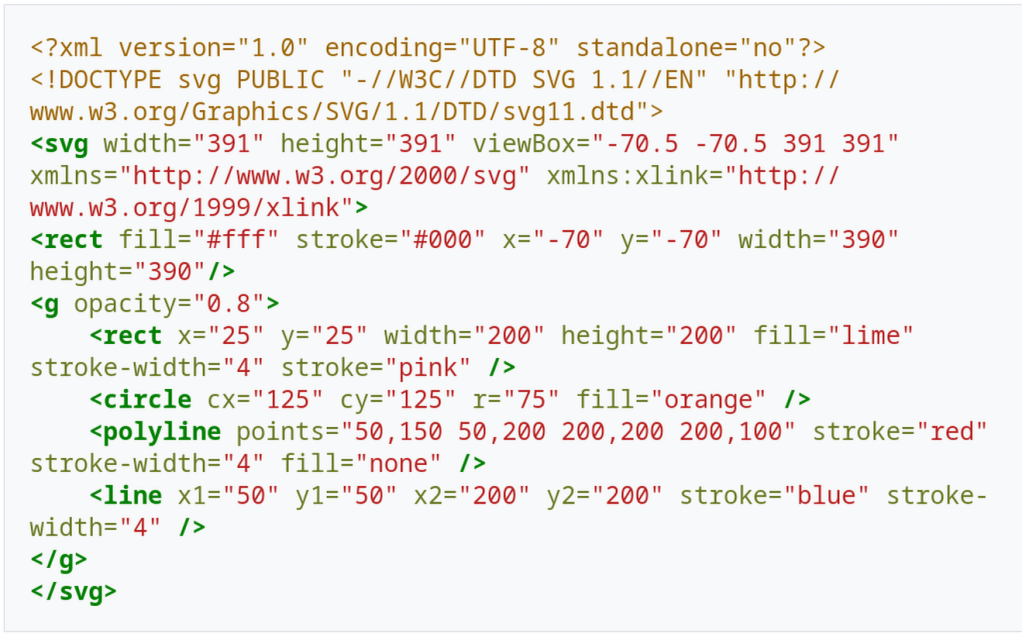
\includegraphics[width=0.6\textwidth]{figure_svg.png}
        \caption{Exemple du contenu d'un fichier .svg}
    \end{figure}
\section{Apprentissage automatique }

	\subsection{Apprentissage automatique}
	%TODO
		
	 	\subsubsection*{Supervisé}
	 	%TODO
	
	 	\subsubsection{Non supervisé}
	 	%TODO
	 	
	\subsection{Apprentissage profond}
	%TODO
	
		\subsubsection{Introduction aux réseaux de neurones}
		%TODO
		
		\subsubsection{Réseaux de neurones multicouches}
		%TODO
		
		\subsubsection{Réseaux de neurones multicouches}
		%TODO
				
		\subsubsection{Transformeurs}
		%TODO
			 
			\paragraph{Attention}
			%TODO
			\paragraph{Auto attention}
			%TODO
			\paragraph{Attention croisée}
			%TODO
			
	\subsection{Fonction de perte}
	%TODO
		
	\subsection{Fonction de coût}
	%TODO
		
	\subsection{Fonction d'activation}
	%TODO

\section{Évaluation des résultats}
	
	\subsection{Mean Squared Error (MSE)}
	%TODO
	
	\subsection{Peak Signal-to-Noise Ratio (PSNR)}
	%TODO
	
	\subsection{Learned Perceptual Image Patch Similarity (LPIPS)}
	%TODO
	
	\subsection{Structural Similarity index (SSIM)}
	%TODO

\section{Travaux connexes}
%TODO

	\subsection{Approche algorithmique}
	%TODO
	
		\subsubsection{(Potrace)}
		%TODO
		
	\subsection{Approche d'optimisation}
	%TODO
	
		\subsubsection{(DIFFVG)}
		%TODO
		
		\subsubsection{(LIVE)}
		%TODO
		
	\subsection{Approche d'apprentissage profond}
	%TODO
	
		\subsubsection{IM2VEC}
		%TODO
		
		\subsubsection{SuperSVG	}
		%TODO
		
\section{Problématique}
% TODO

\section{Conclusion}
% TODO

% ============================================================
%   CHAPITRE 2 — APPROCHE PROPOSÉE
% ============================================================
\chapter{Approche Proposée}

\section{Introduction}
% TODO

\section{Dataset et prétraitement}

  \subsection{Le prétraitement des données}

    \subsubsection{Former les paires d'images}
    % TODO — inclure figure 2.1

    \subsubsection{Augmentation de données}
    % TODO — inclure figures 2.2, 2.3, 2.4

\section{Méthode proposée}

  \subsection{Définir les hyperparamètres évalués par les métaheuristiques}

    \subsubsection{L'Algorithme Génétique}
    % TODO — inclure figures 2.5, 2.6

    \subsubsection{Les paramètres à optimiser}
    % TODO

    \subsubsection{Évaluation d'une solution}
    % TODO

  \subsection{Architecture}

    \subsubsection{Sur-échantillonnage (Upsampling)}
    % TODO — inclure figures 2.7, 2.8, 2.9, 2.10, 2.11

    \subsubsection{Sous-échantillonnage (Downsampling)}
    % TODO — inclure figures 2.12, 2.13, 2.14

\section{Conclusion}
% TODO

% ============================================================
%   CHAPITRE 3 — EXPÉRIMENTATIONS ET RÉSULTATS
% ============================================================
\chapter{Expérimentations et Résultats}

\section{Introduction}
% TODO

\section{Environnement de développement}

  \subsection{Hardware}

  \begin{table}[H]
    \centering
    \caption{Spécifications de la machine Kaggle}
    \label{tab:hardware}
    \begin{tabular}{lll}
      \toprule
      \textbf{CPU} & \textbf{Mémoire} & \textbf{GPU} \\
      \midrule
      1,5 GHz & 13 Go RAM + 73,1 Go HDD & Nvidia P100 — 16 Go VRAM \\
      \bottomrule
    \end{tabular}
  \end{table}

  \subsection{Software}
  % TODO : Python, TensorFlow, NumPy, OpenCV

\section{Dataset utilisé}
% TODO — DIV2K, URBAN 100, Set5 — inclure figures 3.1, 3.2

\section{Prétraitement}
% TODO

\section{Évaluation}

  \subsection{Évaluation quantitative}
  % TODO : PSNR + SSIM

  \subsection{Fonction de perte}

  \begin{equation}
    \mathrm{MAE} = \frac{1}{n}\sum_{i=1}^{n}|y_i - \hat{y}_i|
    \label{eq:mae}
  \end{equation}

\section{Paramétrage de l'Algorithme Génétique}

  \begin{itemize}
    \item Taille de population : 10
    \item Nombre de générations : 6
    \item Probabilité de mutation : 0,5
    \item Fonction objective : PSNR
  \end{itemize}

\section{Sous-échantillonnage}

  \subsection{Hyperparamètres avec la métaheuristique (GA)}

  \begin{table}[H]
    \centering
    \caption{Valeurs du PSNR en fonction du nombre de générations}
    \label{tab:ga_psnr}
    \begin{tabular}{cc}
      \toprule
      \textbf{Générations} & \textbf{PSNR (dB)} \\
      \midrule
      3 & 50,079 \\
      6 & 50,219 \\
      \bottomrule
    \end{tabular}
  \end{table}

  \begin{itemize}
    \item Batch size : 19 \quad Kernel size : $3\times3$
    \item Epochs : 27 \quad Nombre de filtres : 64
    \item Nombre de couches : 5
    \item Learning rate : Adam Optimizer ($10^{-4}$ → $10^{-5}$, limite 5000)
  \end{itemize}

  \subsection{Résultats}

    \subsubsection{Résultats quantitatifs}

    \begin{table}[H]
      \centering
      \caption{Résultats du downsampling (Set5) — PSNR / SSIM}
      \label{tab:downsampling}
      \begin{tabular}{cccc}
        \toprule
        \textbf{Dataset} & \textbf{Facteur}
          & \textbf{Notre Modèle} & \textbf{Bicubique} \\
        \midrule
        \multirow{3}{*}{Set5}
          & $\times 2$ & 45,61 / 0,99 & 36,17 / 0,97 \\
          & $\times 3$ & 44,80 / 0,99 & 30,35 / 0,94 \\
          & $\times 4$ & 33,85 / 0,97 & 26,80 / 0,91 \\
        \bottomrule
      \end{tabular}
    \end{table}

    \subsubsection{Résultats qualitatifs}
    % TODO — inclure figures 3.3, 3.4, 3.5

\section{Sur-échantillonnage}

  \subsection{Hyperparamètres}

  \begin{itemize}
    \item Batch size : 16 \quad Kernel size : $3\times3$
    \item Epochs : 250 \quad Nombre de filtres : 128
    \item Nombre de blocs résiduels : 12
    \item Learning rate : Adam Optimizer ($10^{-4}$ → $10^{-5}$, limite 5000)
  \end{itemize}

  % TODO — inclure figures 3.6 et 3.7

  \subsection{Résultats}

    \subsubsection{Résultats quantitatifs}

    \begin{table}[H]
      \centering
      \caption{Comparaison quantitative sur Set5 (PSNR en dB)}
      \label{tab:upsampling}
      \resizebox{\textwidth}{!}{%
      \begin{tabular}{ccccccccc}
        \toprule
        \textbf{Test set} & \textbf{Facteur}
          & \textbf{Bicubic} & \textbf{SRGAN} & \textbf{DRDN}
          & \textbf{EDSAN} & \textbf{CAR} & \textbf{SRCNN} & \textbf{Notre Modèle} \\
        \midrule
        \multirow{3}{*}{Set5}
          & $\times 2$ & 33,66 & -- & 32,95 & 35,25 & 34,38 & 36,66 & 36,71 \\
          & $\times 3$ & 30,39 & -- & 29,18 & 31,48 & --    & 32,75 & 32,20 \\
          & $\times 4$ & 28,42 & 29,40 & 27,35 & 29,80 & 28,42 & 30,49 & 31,498 \\
        \bottomrule
      \end{tabular}}
    \end{table}

    \subsubsection{Résultats qualitatifs}
    % TODO — inclure figures 3.8, 3.9, 3.10, 3.11

\section{Conclusion}
% TODO

% ============================================================
%   CONCLUSION GÉNÉRALE
% ============================================================
\chapter*{Conclusion Générale}
\addcontentsline{toc}{chapter}{Conclusion Générale}
\markboth{Conclusion Générale}{Conclusion Générale}

Au cours de ce projet de fin d'étude, nous avons exploré divers aspects de l'apprentissage
profond et de la vision par ordinateur pour résoudre le problème du redimensionnement des
images.

% TODO : compléter la conclusion générale

% ============================================================
%   BIBLIOGRAPHIE
% ============================================================
\printbibliography[heading=bibintoc, title={Bibliographie}]

% ============================================================
%   ANNEXES  (optionnel)
% ============================================================
% \appendix
% \chapter{Titre de l'annexe A}
% \lipsum[1]

\end{document}
